% main.tex
% Bachelor's Thesis
% ***
%   Information Theoretic Error Bounds on 
%   NISQ Learning Systems
% ***
% 2021-22
% Sankalp Gambhir
% 180260032

\documentclass[
    aspectratio=169,
    xcolor={dvipsnames},
    % handout,
    % draft
]
{beamer} 

% \usetheme[
%     section page = progressbar,
%     progressbar = foot,
%     background = light,
%     block = transparent,
% ]{metropolis}

% setup packages, macros, notes
\newcounter{notes}
\setcounter{notes}{0}
% general formatting and stuff
\usepackage{graphicx}
\usepackage{xcolor}
\usepackage{ragged2e}
\usepackage{ifthen}
\usepackage{lineno}
\usepackage{booktabs}
\usepackage{subcaption}

% subject specific
\usepackage{amsmath, amssymb, amsthm}
\usepackage{physics, physconst, physunits}
\newtheorem{axiom}{Axiom}

% drawing
\usepackage{pstricks}
\usepackage{tikz, tkz-orm, pgfplots}
\usetikzlibrary{arrows,shapes,backgrounds,decorations.markings}
\usetikzlibrary{matrix,positioning,decorations.pathreplacing,calc,tikzmark}
\pgfplotsset{width=7.5cm,compat=1.16}
\usepgfplotslibrary{fillbetween}

% links and citations
\usepackage{hyperref, bookmark}
\hypersetup{hidelinks} % hide boxes around links ew
\usepackage{csquotes}
\usepackage[
    style=numeric,
    sorting=none
]{biblatex}
\addbibresource{biblio.bib}

% notes
\newcommand{\notes}[1]{}

\ifthenelse{\value{notes} > 0}{
    \renewcommand{\notes}[1]{{\textcolor{red}{[Note: #1]}}}
}{}

% actual macros
\newcommand{\reals}{\ensuremath{\mathbb{R}}}
\newcommand{\naturals}{\ensuremath{\mathbb{N}}}
\newcommand{\complex}{\ensuremath{\mathbb{C}}}
\newcommand{\featurespace}{X}
\newcommand{\labelset}{L}


% meta info
\title{
    {\huge Information Theoretic Bounds on Variational Quantum Algorithms} \\
    {\large B.Tech Project II}
    }
\author[sgambhir@iitb.ac.in]{
    Sankalp Gambhir \\ 
    \vspace{1em}
        {
            \normalsize 
            \hspace{0.1em} 
            Advisor:
            Prof. Sai Vinjanampathy
        }
    \vspace{-1.3em}
}
\date{\today}

\begin{document}

    % title page title page
    \maketitle

    \begin{frame}
        \frametitle{Outline}
    
        \begin{itemize}
            \item Noisy Intermediate-Scale Quantum Systems
            \item NISQy Problems and NISQy Solutions
            \item Variational Quantum Algorithms
            \item Information Theoretic Bounds \emph{(Our results)}
        \end{itemize}
    
    \end{frame}

    % % why qc?
    % % problems with it
    % \input{sections/qc}

    % nisq
    % what can it do?
    \section{NISQ Systems}
    % nisq.tex

% what is nisq
\begin{frame}
    \frametitle{Noisy Intermediate-Scale Quantum Devices}

    \begin{itemize}[<+->]
        \item Near term devices
        \item Not large enough to do error checking and correction --- `noisy'
        \item Few hundred qubits expected --- `intermediate-scale'
        \item Low coherence times
    \end{itemize}

    \notes{These properties leave devices manufacturable in the forseeable future
    unable to live up to the `quantum hype', atleast in a purist's mind. }

\end{frame}

% where can it work
\begin{frame}
    \frametitle{NISQ Devices --- Utility}

    What are NISQ devices good for then?

    \pause

    \begin{itemize}
        \item Computations resilient to noise
        \item Computations with low processing times
    \end{itemize}

    \pause

    \notes{This suggests, rather than using these devices for independent computation,
    perhaps it's better to use them to run subroutines.} 
    %
    Any actual examples to speak of?

\end{frame}

\begin{frame}

    \begin{itemize}
        \item Quantum Approximate Optimization Algorithms (QAOAs)
        \item Quantum Variational Eigensolvers (QVEs)
        \item Ground State Estimation
        \item Polynomial Unconstrained Binary Optimization (PUBO)
                \footfullcite{bittel2021trainingvqa}
                \notes{H is a polynomial of the variables, which take 0/1}
    \end{itemize}


\end{frame}


    % vqa
    % what can you do with a subsystem
    % examples of solvable problems
    % hardness of classical optimization
    \section{Quantum Bandaid}
    % problems.tex

\begin{frame}
    \frametitle{Fixing the leaks}

    \notes{If we claim it is not capable of independent computation, then we don't make it do independent computation}

    \begin{center}
        \emph{\textcolor{Periwinkle}{Use as a subroutine!}}
    \end{center}

    % add VQA tradeoff diagram
    \begin{center}
        \vspace{1em}
        \begin{figure}
            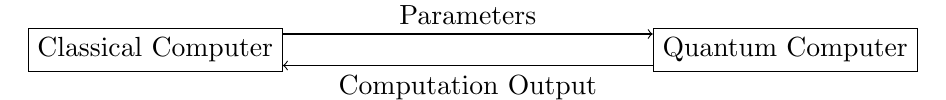
\begin{tikzpicture}[node distance = 8cm]
                \node[draw, rectangle] (C) {Classical Computer};
                \node[draw, rectangle, right of=C] (Q) {Quantum Computer};
	
                
                \begin{scope}[transform canvas={yshift=0.2cm}]
                    \draw[->] (C) -- node[above, midway] {Parameters} (Q);
                \end{scope}
                
                \begin{scope}[transform canvas={yshift=-0.2cm}]
                    \draw[->] (Q) -- node[below, midway] {Computation Output} (C);
                \end{scope}
            \end{tikzpicture}
        \end{figure}
        \vspace{1em}
    \end{center}

\end{frame}

\begin{frame}
    \frametitle{Quantum Bandaid}

    Tides us over while people look for exotic materials and configurations to
    attain reasonable coherence!

    \begin{itemize}
        \item[\textcolor{OliveGreen}{\checkmark}] Computational efficiency of a quantum computer
        \item[\textcolor{OliveGreen}{\checkmark}] Control efficiency of a classical system
        \item[\textcolor{OliveGreen}{\checkmark}] Allows alternate explorations for quantum supremacy
    \end{itemize}

\end{frame}

\begin{frame}
    \frametitle{A Solution}

    \begin{center}
        \textcolor{Periwinkle}{\large Variational Quantum Algorithms \footfullcite{cerezo2021vqa}}

        \begin{figure}
            \includegraphics[width=0.4\textwidth]{figures/vqaapp.pdf}
        \end{figure}
    \end{center}

\end{frame}

    % % classification problem
    % % classical optimization is hard
    % % but nisq compatible?
    % % lead up to vqa
    % % classical.tex

% take classification as a case study
\begin{frame}
    \frametitle{(Supervised) Classification Problem}

    Given a set of input vectors with labels \({\vec{x_i}, y_i}\), learn a
    model, and attempt to predict the labels for arbitrary inputs.
    \footnote{Image: \texttt{User:ZackWeinberg} on Wikimedia Commons, CC BY-SA 3.0}

    % add diagram TODO
    \begin{figure}
        \includegraphics[width=0.4\textwidth]{figures/sephyper.png}
    \end{figure}

\end{frame}

% svm
\begin{frame}
    \frametitle{Support Vector Machines (SVM)}

    Support Vector Machine or Maximum Margin Classifier attempts to find a
    separating plane between labels and optimizes the margin, i.e., distance
    from inputs on either side to it.
    \footnote{Image: \texttt{User:Larhmam} on Wikimedia Commons, CC BY-SA 3.0}

    \begin{multicols}{2}
        % svm fig
        \begin{figure}
            \includegraphics[width=0.4\textwidth]{figures/svmmargin.png}
        \end{figure}
        %
        Hyperplane characterized by a normal vector and a bias \((\vecw, b) \in
        \reals^{n+1}\).
        \begin{gather*}
            \innerproductabstract{\vecw}{\vec{x_i}} + b \geq 1 \text{ if } y_i = 1~, \text{and}\\
            \innerproductabstract{\vecw}{\vec{x_i}} + b \leq -1 \text{ if } y_i = -1~.
        \end{gather*}

        We minimize

        \begin{equation*}
            \mathcal{L}(\vecw, \vec{\alpha}) = \frac{1}{2} \innerprod{\vecw}{\vecw} + \sum_i \alpha_i \left[y_i \cdot \innerprod{\vecw}{\vec{x_i}}\right]~.
        \end{equation*}
    \end{multicols}

\end{frame}

% optimization is hard
\begin{frame}
    \frametitle{Optimization is hard}

    Common techniques --- gradient descent, Hessian-based descent, etc.
    %
    Lots of linear algebraic computation! 

    Matrix multiplication: \(\order{n^{2.37}}\)

    How many dimensions do we have? Consider a simple case of classifying
    \(200\times 200\) sized images, 40,000 dimensional linear algebra!

\end{frame}

% could quantum possibly help?
\begin{frame}
    \frametitle{Quantum Relief?}

    Qubits scale exponentially in the amount of information they can contain. An
    n-qubit state can carry information equivalent to \(\sim 2^n\) complex numbers!

    \pause

    \begin{figure}
        \centering
        \begin{subfigure}{0.45\textwidth}
            \centering
            \includegraphics[width=0.5\textwidth]{figures/blochsphere.png}
        \end{subfigure}
        \pause
        \begin{subfigure}{0.45\textwidth}
            \centering
            \begin{gather*}
                \begin{bmatrix}
                    c_{1,1} & c_{1,2} & \ldots & c_{1,2^n} \\
                    c_{2,1} & c_{2,2} & \ldots & c_{2,2^n} \\
                    \vdots & \ddots & \ddots & \vdots \\
                    c_{2^n,1} & c_{2^n,2} & \ldots & c_{2^n,2^n}
                \end{bmatrix}
            \end{gather*}
        \end{subfigure}
    \end{figure}

    \pause

    The scale of computation is suddenly reduced. Instead of 40,000 dimension
    classical computation, we may only need \(\lceil{\log_2 (40000)}\rceil = 16\)
    qubit sized computation systems.

\end{frame}

% yes, vqas
\begin{frame}
    \frametitle{Quantum, sure, but NISQ?}

    \begin{itemize}
        \item In the near term, it seems the required number of qubits to outpace
                classical computers may not be out of reach.
        \item But can we reliably perform those computations on our quantum
                computers?
        \item Short coherence times make this impossible to do directly.
    \end{itemize}

    \pause

    Perhaps the constrained calculations can be processed as a subroutine? Yes,
    with \emph{Variational Quantum Algorithms}!

\end{frame}


    % vqa
    % components
    % pqc
    % dla
    % qlt
    \section{Variational Quantum Algorithms}
    % vqa.tex

% definition
Hello. \cite{bharti2021noisy}. \notes{Write this section ig}. \notes{borrow
citations from K Bharti}.

% hybrid diagram

\subsection{Building Blocks}

\subsubsection{Objective Function}

\subsubsection{Parametrised Quantum Circuits}
% pqc
% expressiveness of pqc
Expressiveness \cite{larocca2021theory}.

\subsubsection{Measurement}

\subsubsection{Parameter Optimisation}

    % % info theory
    % % why limit
    % % qoc
    % % limits on svm
    % % experiments
    % % infolim.tex

% why is there a limit?
\begin{frame}
    \frametitle{Information Theoretic Limits}

    
    \begin{multicols}{2}
        \begin{figure}
            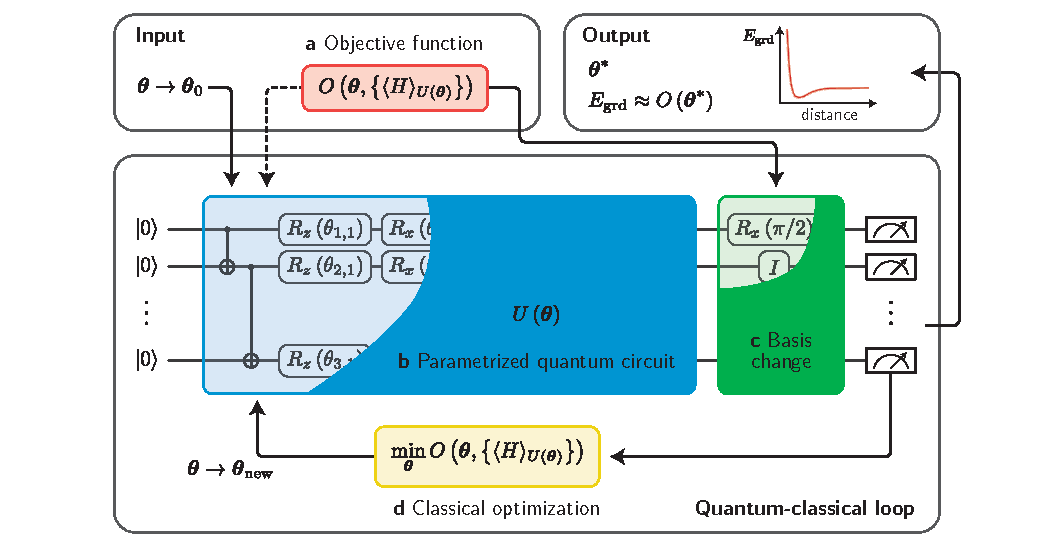
\includegraphics[width=0.55\textwidth]{figures/vqaarch.pdf}
        \end{figure}
        %
        The classical system transferring information about the parameters to
        the PQC has a limit on how much information it can transfer in a given
        time \(T\) given by
        \begin{gather*}
            b = T\Delta\Omega\kappa_s
        \end{gather*}
        where \(\Delta\Omega\) is the channel bandwidth and \(\kappa_s\) is the
        bit depth of the control signal (amount of information \emph{per}
        trasnfer).
    \end{multicols}{2}

\end{frame}

% summary of bounds on qoc
\begin{frame}
    \frametitle{Example --- Bounds on Quantum Optical Control}

    For the specific example of a control pulse for a quantum system

    \begin{gather*}
        \dot{\rho} = \mathcal{L}(\rho, \gamma(t))~,
    \end{gather*}

    where \(\rho\) is the state density matrix, \(\mathcal{L}\) is the
    Liouvillian operator, and \(\gamma(t)\) is the control pulse. We have the
    Hamiltonian

    \begin{gather*}
        \hamiltonian = \hamiltonian_D + \gamma(t)\cdot \hamiltonian_C~.
    \end{gather*}

\end{frame}

\begin{frame}
    \frametitle{Example --- Bounds on Quantum Optical Control}
    
    We have

    \begin{gather*}
        \kappa_s = \log (1 + \frac{\Delta\gamma}{\delta\gamma})~,
    \end{gather*}

    where \(\Delta\gamma\) and \(\delta\gamma\) are the maximum and minimum
    variation in the control field.

    We have the error bound \cite{lloyd2014information} \(\norm*{\rho-\rho_*} >
    \epsilon\), with

    \begin{gather*}
        \epsilon \geq 2^{-\frac{T\Delta\Omega\kappa_s}{\dimD_\polyreachable}}~,
    \end{gather*}

    where \(\dimD_\polyreachable\) is the dimension of the relevant
    (polynomially reachable) space of density matrices.

    We intend to employ a similar technique to establish bounds on PQC errors.

\end{frame}

% bounds on qsvm

% proposed bounds on pqc

    % info theory
    % why limit
    % qoc
    % ansatz expressibility
    % trainability tradeoff
    % limits of expressibility
    \section{Information Theoretic Bounds}
    % infolim.tex

% why is there a limit?
\begin{frame}
    \frametitle{Information Theoretic Limits}

    
    \begin{multicols}{2}
        \begin{figure}
            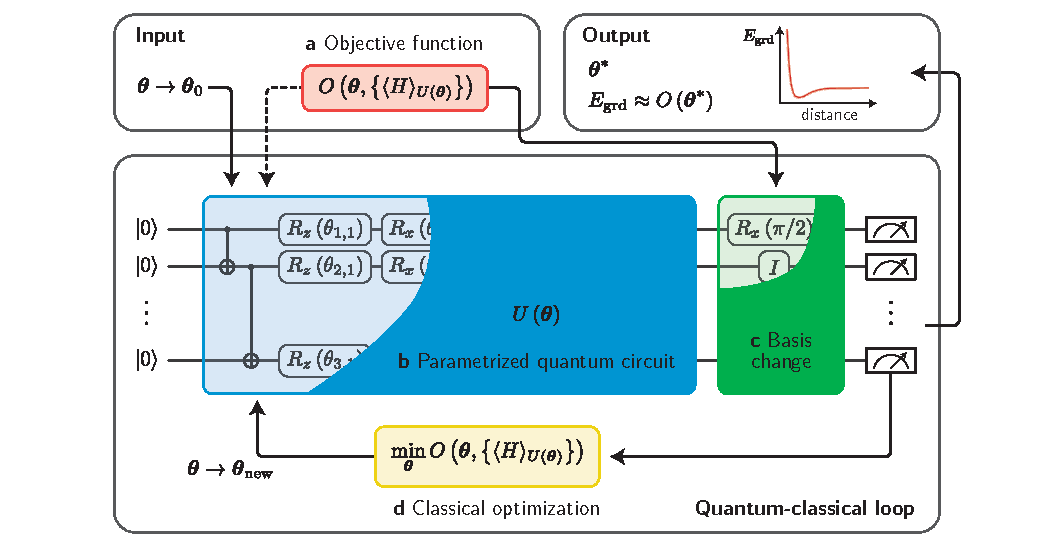
\includegraphics[width=0.55\textwidth]{figures/vqaarch.pdf}
        \end{figure}
        %
        The classical system transferring information about the parameters to
        the PQC has a limit on how much information it can transfer in a given
        time \(T\) given by
        \begin{gather*}
            b = T\Delta\Omega\kappa_s
        \end{gather*}
        where \(\Delta\Omega\) is the channel bandwidth and \(\kappa_s\) is the
        bit depth of the control signal (amount of information \emph{per}
        trasnfer).
    \end{multicols}{2}

\end{frame}

% summary of bounds on qoc
\begin{frame}
    \frametitle{Example --- Bounds on Quantum Optical Control}

    For the specific example of a control pulse for a quantum system

    \begin{gather*}
        \dot{\rho} = \mathcal{L}(\rho, \gamma(t))~,
    \end{gather*}

    where \(\rho\) is the state density matrix, \(\mathcal{L}\) is the
    Liouvillian operator, and \(\gamma(t)\) is the control pulse. We have the
    Hamiltonian

    \begin{gather*}
        \hamiltonian = \hamiltonian_D + \gamma(t)\cdot \hamiltonian_C~.
    \end{gather*}

\end{frame}

\begin{frame}
    \frametitle{Example --- Bounds on Quantum Optical Control}
    
    We have

    \begin{gather*}
        \kappa_s = \log (1 + \frac{\Delta\gamma}{\delta\gamma})~,
    \end{gather*}

    where \(\Delta\gamma\) and \(\delta\gamma\) are the maximum and minimum
    variation in the control field.

    We have the error bound \cite{lloyd2014information} \(\norm*{\rho-\rho_*} >
    \epsilon\), with

    \begin{gather*}
        \epsilon \geq 2^{-\frac{T\Delta\Omega\kappa_s}{\dimD_\polyreachable}}~,
    \end{gather*}

    where \(\dimD_\polyreachable\) is the dimension of the relevant
    (polynomially reachable) space of density matrices.

    We intend to employ a similar technique to establish bounds on PQC errors.

\end{frame}

% bounds on qsvm

% proposed bounds on pqc

    \begin{frame}{References}
        \printbibliography
    \end{frame}
\end{document}